\let\negmedspace\undefined
\let\negthickspace\undefined
\documentclass[journal,12pt,onecolumn]{IEEEtran}
\usepackage{cite}
\usepackage{amsmath,amssymb,amsfonts,amsthm}
\usepackage{algorithmic}
\usepackage{graphicx}
\graphicspath{{./figs/}}
\usepackage{textcomp}
\usepackage{xcolor}
\usepackage{txfonts}
\usepackage{listings}
\usepackage{enumitem}
\usepackage{mathtools}
\usepackage{gensymb}
\usepackage{comment}
\usepackage{caption}
\usepackage[breaklinks=true]{hyperref}
\usepackage{tkz-euclide} 
\usepackage{listings}
\usepackage{gvv}                                        
%\def\inputGnumericTable{}                                 
\usepackage[latin1]{inputenc}     
\usepackage{xparse}
\usepackage{color}                                            
\usepackage{array}                                            
\usepackage{longtable}                                       
\usepackage{calc}                                             
\usepackage{multirow}
\usepackage{multicol}
\usepackage{hhline}                                           
\usepackage{ifthen}                                           
\usepackage{lscape}
\usepackage{tabularx}
\usepackage{array}
\usepackage{float}
\newtheorem{theorem}{Theorem}[section]
\newtheorem{problem}{Problem}
\newtheorem{proposition}{Proposition}[section]
\newtheorem{lemma}{Lemma}[section]
\newtheorem{corollary}[theorem]{Corollary}
\newtheorem{example}{Example}[section]
\newtheorem{definition}[problem]{Definition}
\newcommand{\BEQA}{\begin{eqnarray}}
\newcommand{\EEQA}{\end{eqnarray}}
\newcommand{\define}{\stackrel{\triangle}{=}}
\theoremstyle{remark}
\newtheorem{rem}{Remark}

\begin{document}
\title{
ASSIGNMENT 1: GATE 2010 \\
IN: INSTRUMENTATION ENGINEERING}
\author{EE25BTECH11062 - Vivek K Kumar}
\maketitle
\renewcommand{\thefigure}{\theenumi}
\renewcommand{\thetable}{\theenumi}
\begin{enumerate}

\item The infinite series $f\brak{x} = x - \frac{x^3}{3!} + \frac{x^5}{5!} - \frac{x^7}{7!} \dots \dots \infty$ converges to

\hfill{\brak{\text{GATE IN 2010}}}
\begin{enumerate}
\begin{multicols}{4}
\item $\cos\brak{x}$
\item $\sin\brak{x}$
\item $\sinh\brak{x}$
\item $e^x$
\end{multicols}
\end{enumerate}

\item The diameters of $10000$ ball bearings were measured. The mean diameter and standard deviation were found to be $10mm$ and $0.05mm$ respectively. Assuming Gaussian distribution of measurements, it can be expected that the number of measurements more than $ 10.15 mm$ will be

\hfill{\brak{\text{GATE IN 2010}}}
\begin{enumerate}
\begin{multicols}{4}
\item $230$
\item $115$
\item $15$
\item $2$
\end{multicols}
\end{enumerate}

\item A person weighing $60kg$ receives radiation energy of $0.3J$ over the entire body. The dose of radiation absorbed \brak{\text{in rad}} is

\hfill{\brak{\text{GATE IN 2010}}}
\begin{enumerate}
\begin{multicols}{4}
\item $0.005$ rad
\item $0.1$ rad
\item $0.3$ rad
\item $0.5$ rad
\end{multicols}
\end{enumerate}

\item $u\brak{t}$ represents the unit step function. The Laplace transform of $u\brak{t - \tau}$ is

\hfill{\brak{\text{GATE IN 2010}}}
\begin{enumerate}
\begin{multicols}{4}
\item $\frac{1}{s\tau}$
\item $\frac{1}{s-\tau}$
\item $\frac{e^{-s\tau}}{s}$
\item $e^{-s\tau}$
\end{multicols}
\end{enumerate}

\item A measurement system with input $x\brak{t}$ and output $y\brak{t}$ is described by the differential equation $3\frac{dy}{dt} + 5y = 8x$. The static sensitivity of the system is

\hfill{\brak{\text{GATE IN 2010}}}
\begin{enumerate}
\begin{multicols}{4}
\item $0.60$
\item $1.60$
\item $1.67$
\item $2.67$
\end{multicols}
\end{enumerate}

\item Poisson's ratio of a metal is $0.35$. Neglecting piezo-resistance effect, the gage factor of a strain gage made of this metal is

\hfill{\brak{\text{GATE IN 2010}}}
\begin{enumerate}
\begin{multicols}{4}
\item $0.65$
\item $1$
\item $1.35$
\item $1.70$
\end{multicols}
\end{enumerate}

\item Match the following:
\begin{table}[H]
    \centering\normalsize
    \begin{tabular}{|m{18em}|m{18em}|}
    \hline
        P. Radiation Pyrometer & W. Angular velocity measurement  \\
    \hline
        Q. Dall tube & X. Vaccum pressure measurement \\
    \hline
        R. Pirani gauge & Y. Flow measurement \\
    \hline
        S. Gyroscope & Z. Temperature measurement \\
        \hline
    \end{tabular}
    \caption*{}
    \label{tab:Q7}
\end{table}

\hfill{\brak{\text{GATE IN 2010}}}

\begin{enumerate}
\begin{multicols}{2}
\item P-Z, Q-W, R-X, S-Y
\item P-Z, Q-Y, R-X, S-W
\item P-W, Q-X, R-Y, S-Z
\item P-Z, Q-X, R-W, S-Y
\end{multicols}
\end{enumerate}

\item In a pulse code modulated \brak{\text{PCM}} signal sampled at $f_s$ and encoded into an $n$-bit code, the minimum bandwidth required for faithful reconstruction is

\hfill{\brak{\text{GATE IN 2010}}}
\begin{enumerate}
\begin{multicols}{4}
\item $2nf_s$
\item $nf_s$
\item $\frac{nf_s}{2}$
\item $f_s$
\end{multicols}
\end{enumerate}

\item A beam of unpolarized light is first passed through a linear polarizer and then through a quarter-wave plate. The emergent beam is

\hfill{\brak{\text{GATE IN 2010}}}
\begin{enumerate}
\begin{multicols}{2}
\item unpolarized
\item linearly polarized
\item circularly polarized
\item elliptically polarized
\end{multicols}
\end{enumerate}

\item $f\brak{x},$ shown in the adjoining figure is represented by
\begin{align*}
f\brak{x} = a_0 + \sum_{n=1}^{\infty}\cbrak{a_n \cos\brak{nx} + b_n \sin\brak{mx}}
\end{align*}
The value of $a_0$ is
\begin{figure}[H]
    \centering
    \includegraphics[width=0.7\columnwidth]{q10}
    \caption*{}
    \label{fig:Q10}
\end{figure}

\hfill{\brak{\text{GATE IN 2010}}}
\begin{enumerate}
\begin{multicols}{4}
\item 0
\item $\frac{\pi}{2}$
\item $\pi$
\item $2\pi$
\end{multicols}
\end{enumerate}

\item  The PMMC ammeter A in the adjoining figure has a range of 0 to 3 mA. When switch S1 is opened, the pointer of the ammeter swings to the 1 mA mark, returns and settles at 0.9 mA. The meter is
\begin{figure}[H]
    \centering
    \includegraphics[width = 0.7\columnwidth]{q11}
    \caption*{}
    \label{fig:Q11}
\end{figure}

\hfill{\brak{\text{GATE IN 2010}}}
\begin{enumerate}
\item  critically damped and has a coil resistance of 100 $\ohm$
\item critically damped and has a coil resistance of 200 $\ohm$
\item under damped and has a coil resistance of 100 $\ohm$
\item under damped and has a coil resistance of 200 $\ohm$
\end{enumerate}

\item The open loop transfer function of a unity gain feedback system is given by: 
\begin{align*}
G\brak{s} = \frac{k\brak{s+3}}{\brak{s+1}\brak{s+2}}
\end{align*}
The range of positive values of k for which the closed loop system will remain stable is:

\hfill{\brak{\text{GATE IN 2010}}}
\begin{enumerate}
\begin{multicols}{2}
\item $1 < k < 3$
\item $0 < k < 10$
\item $5 < k < \infty$
\item $0 < k < \infty$
\end{multicols}
\end{enumerate}

\item A real $n \times n$ matrix $A = [a_{ij}]$ is defined as follows:
\begin{align*}
    a_{ij} &=i, if \text{ i = j}; \\
    &= 0, \text{ otherwise}
\end{align*}
The summation of all eigenvalues of A is

\hfill{\brak{\text{GATE IN 2010}}}
\begin{enumerate}
\begin{multicols}{4}
\item $n\brak{n+1}/2$
\item $n\brak{n-1}/2$
\item $\frac{n\brak{n+1}\brak{2n+1}}{6}$
\item $n^2$
\end{multicols}
\end{enumerate}

\item The contour C in the adjoining figure is described by $x^2 + y^2 = 16$.

\begin{minipage}{0.45\columnwidth}
\begin{figure}[H]
    \centering
    \includegraphics[width = 0.6\columnwidth]{q14}
    \caption*{}
    \label{fig:Q14}
\end{figure}
\end{minipage}
\hspace{0.05\columnwidth}
\begin{minipage}{0.45\columnwidth}
The value of 
\begin{align*}
\oint\limits_{C} \frac{z^2+8}{0.5z - 1.5j} dz
\end{align*}
is \brak{\text{Note: $j = \sqrt{-1}$}}
\end{minipage}

\hfill{\brak{\text{GATE IN 2010}}}
\begin{enumerate}
\begin{multicols}{4}
\item $-2\pi j$
\item $2\pi j$
\item $4\pi j$
\item $-4\pi j$
\end{multicols}
\end{enumerate}

\item In the dc circuit shown in the adjoining figure, the node voltage $V_2$ at steady state is
\begin{figure}[H]
    \centering
    \includegraphics[width = 0.7\columnwidth]{q15}
    \caption*{}
    \label{fig:Q15}
\end{figure}

\hfill{\brak{\text{GATE IN 2010}}}
\begin{enumerate}
\begin{multicols}{4}
\item 0 V
\item 1 V
\item 2 V
\item 3 V
\end{multicols}
\end{enumerate}

\item A 100 $\ohm$, 1 W resistor and a 800 $\ohm$, 2 W resistor are connected in series. The maximum dc voltage that can be applied continuously to the series circuit without exceeding the power limit of any of the resistors is

\hfill{\brak{\text{GATE IN 2010}}}
\begin{enumerate}
\begin{multicols}{4}
\item 90 V
\item 50 V
\item 45 V
\item 40 V
\end{multicols}
\end{enumerate}

\item The seismic mass of an accelerometer oscillates sinusoidally at 100 Hz with a maximum displacement of 10 mm from its mean position. The peak acceleration of the seismic mass is

\hfill{\brak{\text{GATE IN 2010}}}
\begin{enumerate}
\begin{multicols}{4}
\item $3947.84 \, m/s^2$
\item $3141.50 \, m/s^2$
\item $314.15 \, m/s^2$
\item $100.00 \, m/s^2$
\end{multicols}
\end{enumerate}

\item In the ideal opamp circuit given in the adjoining figure, the value of $R_f$ is varied from 1 k$\ohm$ to 100 k$\ohm$. The gain $G = \brak{v_o/v_i}$ will
\begin{figure}[H]
    \centering
    \includegraphics[width = 0.7\columnwidth]{q18}
    \caption*{}
    \label{fig:Q18}
\end{figure}

\hfill{\brak{\text{GATE IN 2010}}}
\begin{enumerate} 
\begin{multicols}{2}
    \item remain constant at +1
    \item remain constant at -1
    \item vary as $-\brak{R_f/10,000}$
    \item vary as $\brak{1+R_f/10,000}$
\end{multicols} \end{enumerate}


\item A signal with frequency components 50 Hz, 100 Hz and 200 Hz only is sampled at 150 samples/s. The ideally reconstructed signal will have frequency component\brak{\text{s}} of

\hfill{\brak{\text{GATE IN 2010}}}\begin{enumerate} \begin{multicols}{2}
    \item 50 Hz only
    \item 75 Hz only
    \item 50 Hz and 75 Hz
    \item 50 Hz, 75 Hz and 100 Hz
\end{multicols} \end{enumerate}

\item The subroutine SBX given below is executed by an 8085 processor. The value in the accumulator immediately after the execution of the subroutine will be:
\begin{verbatim}
SBX: MVI A, 99h
     ADI 11h
     MOV C, A
     RET
\end{verbatim}

\hfill{\brak{\text{GATE IN 2010}}}\begin{enumerate} \begin{multicols}{4}
    \item 00h
    \item 11h
    \item 99h
    \item AAh
\end{multicols} \end{enumerate}



\item The integral $\int\limits_{-\infty}^{\infty} \delta\brak{t - \pi/6} 6 \sin\brak{t} dt$ evaluates to

\hfill{\brak{\text{GATE IN 2010}}}\begin{enumerate} \begin{multicols}{4}
    \item 6
    \item 3
    \item 1.5
    \item 0
\end{multicols} \end{enumerate}



\item The deflection angle of the pointer of an ideal moving iron ammeter is $20\degree$ for 1.0 ampere dc current. If a current of $3 \sin\brak{314t}$ amperes is passed through the ammeter then the deflection angle is

\hfill{\brak{\text{GATE IN 2010}}}\begin{enumerate} \begin{multicols}{4}
    \item $0\degree$
    \item $42\degree$
    \item $60\degree$
    \item $90\degree$
\end{multicols} \end{enumerate}



\item An 8-bit DAC is interfaced with a microprocessor having 16 address lines \brak{A_0\dots A_{15}} as shown in the adjoining figure. A possible valid address for this DAC is
\begin{figure}[H]
    \centering
    \includegraphics[width = 0.7\columnwidth]{q23}
    \caption*{}
    \label{fig:Q23}
\end{figure}

\hfill{\brak{\text{GATE IN 2010}}}\begin{enumerate} \begin{multicols}{4}
    \item 3000h
    \item 4FFFh
    \item AFFFh
    \item C000h
\end{multicols} 
\end{enumerate}

\item $H\brak{z}$ is a discrete rational transfer function. To ensure that both $H\brak{z}$ and its inverse are stable its

\hfill{\brak{\text{GATE IN 2010}}}\begin{enumerate}
    \item poles must be inside the unit circle and zeros must be outside the unit circle.
    \item poles and zeros must be inside the unit circle.
    \item poles and zeros must be outside the unit circle.
    \item poles must be outside the unit circle and the zeros should be inside the unit circle.
 \end{enumerate}



\item The output voltage of a transducer with an output resistance of 10 k$\ohm$ is connected to an amplifier. The minimum input resistance of the amplifier so that the error in recording the transducer output does not exceed 2\% is

\hfill{\brak{\text{GATE IN 2010}}}
\begin{enumerate}
\begin{multicols}{4}
    \item 10 k$\ohm$
    \item 49 k$\ohm$
    \item 490 k$\ohm$
    \item 1.2 M$\ohm$
\end{multicols} \end{enumerate}



\item X and Y are non-zero square matrices of size $n \times n$. If $XY=0_{n \times n}$ then

\hfill{\brak{\text{GATE IN 2010}}}\begin{enumerate} \begin{multicols}{2}
    \item $\abs{X}=0$ and $\abs{Y}\neq0$
    \item $\abs{X}\neq0$ and $\abs{Y}=0$
    \item $\abs{X}=0$ and $\abs{Y}=0$
    \item $\abs{X}\neq0$ and $\abs{Y}\neq0$
\end{multicols} \end{enumerate}



\item Consider the differential equation $\frac{dy}{dx} + y = e^x$ with $y\brak{0} = 1$. The value of $y\brak{1}$ is

\hfill{\brak{\text{GATE IN 2010}}}
\begin{enumerate} \begin{multicols}{4}
    \item $e + e^{-1}$
    \item $\frac{1}{2}\brak{e - e^{-1}}$
    \item $\frac{1}{2}\brak{e + e^{-1}}$
    \item $2\brak{e - e^{-1}}$
\end{multicols} \end{enumerate}



\item The electric charge density in the region $R\colon x^2+y^2 \le 1, y \le 0$ is given as $\sigma\brak{x,y} = 1 \, C/m^2$, where x and y are in meters. The total charge \brak{\text{in coulomb}} contained in the region R is

\hfill{\brak{\text{GATE IN 2010}}}\begin{enumerate} \begin{multicols}{4}
    \item $4\pi$
    \item $2\pi$
    \item $\pi/2$
    \item 0
\end{multicols} \end{enumerate}



\item The input $x\brak{t}$ and the corresponding output $y\brak{t}$ of a system are related by $y\brak{t} = \int_{-\infty}^{5t} x\brak{\tau} d\tau$. The system is

\hfill{\brak{\text{GATE IN 2010}}}\begin{enumerate} \begin{multicols}{2}
    \item time invariant and causal
    \item time invariant and noncausal
    \item time variant and noncausal
    \item time variant and causal
\end{multicols} \end{enumerate}



\item A digital filter having a transfer function $H\brak{z} = \frac{p_0 + p_1 z^{-1} + p_3 z^{-3}}{1 + d_3 z^{-3}}$ is implemented using Direct Form-I and Direct Form-II realizations of IIR structure. The number of delay units required in Direct Form-I and Direct Form-II realizations are, respectively

\hfill{\brak{\text{GATE IN 2010}}}\begin{enumerate} \begin{multicols}{4}
    \item 6 and 6
    \item 6 and 3
    \item 3 and 3
    \item 3 and 2
\end{multicols} \end{enumerate}



\item The velocity v \brak{\text{in m/s}} of a moving mass, starting from rest, is given as $\frac{dv}{dt} = v+t$. Using Euler forward difference method \brak{\text{also known as Cauchy-Euler method}} with a step size of 0.1 s, the velocity at 0.2 s evaluates to

\hfill{\brak{\text{GATE IN 2010}}}\begin{enumerate} \begin{multicols}{4}
    \item 0.01 m/s
    \item 0.1 m/s
    \item 0.2 m/s
    \item 1 m/s
\end{multicols} \end{enumerate}



\item The rotor of the control transformer of a synchro pair gives a maximum voltage of 1.0 V at a particular position of the rotor of the control transmitter. The transmitter rotor is now rotated by $30\degree$ anticlockwise keeping the transformer rotor stationary. The transformer rotor voltage for this position is

\hfill{\brak{\text{GATE IN 2010}}}\begin{enumerate} \begin{multicols}{4}
    \item 1.0 V
    \item 0.866 V
    \item 0.5 V
    \item 0 V
\end{multicols} \end{enumerate}



\item The matched transistors Q1 and Q2 shown in the adjoining figure have $\beta = 100$. Assuming the base-emitter voltages to be 0.7 V, the collector-emitter voltage $V_2$ of the transistor Q2 is
\begin{figure}[H]
    \centering
    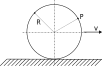
\includegraphics[width = 0.7\columnwidth]{q33}
    \caption*{}
    \label{fig:Q33}
\end{figure}

\hfill{\brak{\text{GATE IN 2010}}}\begin{enumerate} \begin{multicols}{4}
    \item 33.9 V
    \item 27.8 V
    \item 16.2 V
    \item 0.7 V
\end{multicols} \end{enumerate}

\item The volume of a cylinder is computed from measurements of its height \brak{\text{h}} and diameter \brak{\text{d}}. A set of several measurements of height has an average value of 0.2 m and a standard deviation of 1\%. The average value obtained for the diameter is 0.1 m and the standard deviation is 1\%. Assuming the errors in the measurements of height and diameter are uncorrelated, the standard deviation of the computed volume is

\hfill{\brak{\text{GATE IN 2010}}}\begin{enumerate} \begin{multicols}{4}
    \item 1.00\%
    \item 1.73\%
    \item 2.23\%
    \item 2.41\%
\end{multicols} \end{enumerate}



\item A thermocouple based temperature measurement system is shown in the adjoining figure. Relevant thermocouple emf data \brak{\text{in mV}} is given below. The cold junction is kept at $0\degree C$. The temperature is $30\degree C$ in the other parts of the system. The emf $V_o$ is measured to be 26.74 mV. The temperature of the hot liquid is
\begin{figure}[H]
    \centering
    \includegraphics[width = 0.7\columnwidth]{q35}
    \caption*{}
    \label{fig:Q35}
\end{figure}
\begin{table}[H]
    \centering\normalsize
    \begin{tabular}{|l|c|c|}
        \hline
        \textbf{Temperature} & \textbf{emf of Chromel-Constantan} & \textbf{emf of Copper-Constantan} \\
        \hline
        $10\degree C$ & 0.591 & 0.391 \\
        \hline
        $20\degree C$ & 1.192 & 0.789 \\
        \hline
        $30\degree C$ & 1.801 & 1.196 \\
        \hline
        $370\degree C$ & 26.549 & 19.027 \\
        \hline
        $380\degree C$ & 27.345 & 19.638 \\
        \hline
    \end{tabular}
    \caption*{}
    \label{tab:Q35}
\end{table}

\hfill{\brak{\text{GATE IN 2010}}}\
\begin{enumerate} \begin{multicols}{4}
    \item $370.0\degree C$
    \item $372.4\degree C$
    \item $376.6\degree C$
    \item $380.0\degree C$
\end{multicols} \end{enumerate}



\item A differential pressure transmitter is used to measure the flow rate in a pipe. Due to aging, the sensitivity of the pressure transmitter is reduced by 5\%. All other aspects of the flow meter remaining constant, change in the sensitivity of the flow measurement is

\hfill{\brak{\text{GATE IN 2010}}}\begin{enumerate} \begin{multicols}{4}
    \item 10.0\%
    \item 5.0\%
    \item 2.5\%
    \item 2.2\%
\end{multicols} \end{enumerate}



\item The asymptotic Bode magnitude plot of a lead network with its pole and zero on the left half of the s-plane is shown in the adjoining figure. The frequency at which the phase angle of the network is maximum \brak{\text{in rad/s}} is
\begin{figure}[H]
    \centering
    \includegraphics[width = 0.7\columnwidth]{q37}
    \caption*{}
    \label{Q37}
\end{figure}

\hfill{\brak{\text{GATE IN 2010}}}
\begin{enumerate} 
\begin{multicols}{4}
    \item $\frac{3}{\sqrt{10}}$
    \item $\frac{1}{\sqrt{20}}$
    \item $\frac{1}{20}$
    \item $\frac{1}{30}$
\end{multicols} \end{enumerate}

\item In an analog single channel cathode ray oscilloscope \brak{\text{CRO}}, the x and y sensitivities are set as 1 ms/div and 1 V/div, respectively. The y-input is connected to a voltage signal $4 \cos\brak{200\pi t - 45\degree}$ V. The trigger source is internal, level chosen is zero and the slope is positive. The display seen on the CRO screen is

\hfill{\brak{\text{GATE IN 2010}}}
\begin{enumerate}
\begin{figure}[H]
\centering
\begin{multicols}{2}
    \item
        \includegraphics[width = 0.5\columnwidth]{38aa}
    \item \includegraphics[width = 0.5\columnwidth]{38ab}
    \item \includegraphics[width = 0.5\columnwidth]{38ac}
    \item \includegraphics[width = 0.5\columnwidth]{38ad}
\end{multicols}
\caption*{}
\label{fig:q38}
\end{figure}
\end{enumerate}

\item A unit ramp input is applied to the system shown in the adjoining figure. The steady state error in its output is
\begin{figure}[H]
    \centering
    \includegraphics[width = 0.7\columnwidth]{q39}
    \caption*{}
    \label{fig:Q39}
\end{figure}

\hfill{\brak{\text{GATE IN 2010}}}\begin{enumerate} \begin{multicols}{4}
    \item 0
    \item 0.5
    \item 1
    \item 2
\end{multicols} \end{enumerate}



\item A unity feedback system has an open loop transfer function $G\brak{s} = \frac{k}{s\brak{s+3}}$. The value of k that yields a damping ratio of 0.5 for the closed loop system is

\hfill{\brak{\text{GATE IN 2010}}}\begin{enumerate} \begin{multicols}{4}
    \item 1
    \item 3
    \item 5
    \item 9
\end{multicols} \end{enumerate}

\item A 4-bit successive approximation type ADC has a full scale value of 15 V. The sequence of the states, the SAR will traverse, for the conversion of an input of 8.15 V is

\hfill{\brak{\text{GATE IN 2010}}}
\begin{figure}[H]
    \centering
    \begin{enumerate} 
    \item \caption*{} \label{41A}\includegraphics[width = 0.7\columnwidth]{41a}
    \item \caption*{} \label{41B}\includegraphics[width = 0.7\columnwidth]{41b}
    \item \caption*{} \label{41C}\includegraphics[width = 0.7\columnwidth]{41c}
    \item \caption*{} \label{41D}\includegraphics[width = 0.7\columnwidth]{41d}
 \end{enumerate}
 \caption*{}
 \label{fig:Q41}
\end{figure}




\item The logic gate circuit shown in the adjoining figure realizes the function
\begin{figure}[H]

    \centering
    \includegraphics[width = 0.7\columnwidth]{q42}
    \caption*{}
    \label{fig:Q42}
\end{figure}

\hfill{\brak{\text{GATE IN 2010}}}\begin{enumerate} \begin{multicols}{2}
    \item XOR
    \item XNOR
    \item Half adder
    \item Full adder
\end{multicols} \end{enumerate}



\item In an 8085 processor, the main program calls the subroutine SUB1 given below. When the program returns to the main program after executing SUB1, the value in the accumulator is
\begin{center}
\begin{verbatim}
Address     Opcode      Mnemonic
2000h       3E 00       SUB1: MVI A, 00h
2002h       CD 05 20          CALL SUB2
2005h       3C          SUB2: INR A
2006h       C9                RET
\end{verbatim}
\end{center}

\hfill{\brak{\text{GATE IN 2010}}}\begin{enumerate} \begin{multicols}{4}
    \item 00
    \item 01
    \item 02
    \item 03
\end{multicols} \end{enumerate}



\item Light coming out of an optical fiber is incident on a plane perpendicular to the fiber axis and 50 mm away from the end of the fiber. The light coming out creates a circular spot that can at most be of 20 mm diameter. Neglecting the diameter of the fiber, the numerical aperture of the fiber is, approximately,

\hfill{\brak{\text{GATE IN 2010}}}\begin{enumerate} \begin{multicols}{4}
    \item 0.14
    \item 0.20
    \item 0.34
    \item 0.40
\end{multicols} \end{enumerate}



\item A solution "P" is put in a spectrophotometer cuvette of optical path length 1 cm. The transmittance is found to be 10\%. Another solution "Q" has a transmittance of 40\% under the same circumstances. If equal volumes of P and Q are mixed together, the transmittance of the resulting solution \brak{\text{assuming the constituents of P and Q do not react with each other}} is, approximately,

\hfill{\brak{\text{GATE IN 2010}}}\begin{enumerate} \begin{multicols}{4}
    \item 15\%
    \item 20\%
    \item 25\%
    \item 30\%
\end{multicols} \end{enumerate}



\item 4-point DFT of a real discrete-time signal $x[n]$ of length 4 is given by $X[k]$, $n=0,1,2,3$ and $k=0,1,2,3$. It is given that $X[0]=5$, $X[1]=1+j1$, $X[2]=0.5$. $X[3]$ and $x[0]$ respectively are

\hfill{\brak{\text{GATE IN 2010}}}
\begin{enumerate} \begin{multicols}{4}
    \item $1-j$, 1.875
    \item $1-j$, 1.500
    \item $1+j$, 1.875
    \item $0.1-j0.1$, 1.500
\end{multicols} 
\end{enumerate}



\item An active filter is shown in the adjoining figure. The dc gain and the 3 dB cut-off frequency of the filter respectively, are, nearly
\begin{figure}[H]
    \centering
    \includegraphics[width = 0.7\columnwidth]{q47}
    \caption*{}
    \label{fig:Q47}
\end{figure}

\hfill{\brak{\text{GATE IN 2010}}}
\begin{enumerate} 
\begin{multicols}{2}
    \item 40 dB, 3.14 kHz
    \item 40 dB, 1.00 kHz
    \item 20 dB, 6.28 kHz
    \item 20 dB, 1.00 kHz
\end{multicols} 
\end{enumerate}


A differential amplifier is constructed using an ideal opamp as shown in the adjoining figure. The values of $R_1$ and $R_2$ are 47 k$\ohm$ and 470 k$\ohm$ respectively.
\begin{figure}[H]
    \centering
    \includegraphics[width = 0.7\columnwidth]{q48}
    \caption*{}
    \label{fig:Q48}
\end{figure}


\item The input impedances seen looking into the terminals $V_1$ and $V_2$, with respect to ground, respectively are

\hfill{\brak{\text{GATE IN 2010}}}\begin{enumerate} \begin{multicols}{2}
    \item 47 k$\ohm$ and 43 k$\ohm$
    \item 47 k$\ohm$ and 47 k$\ohm$
    \item 47 k$\ohm$ and 517 k$\ohm$
    \item 517 k$\ohm$ and 517 k$\ohm$
\end{multicols} \end{enumerate}

\item $V_1$ and $V_2$ are connected to voltage sources having an open circuit output of +1 V each and internal resistances of 13 k$\ohm$ and 3 k$\ohm$ respectively. The output voltage $V_o$ is

\hfill{\brak{\text{GATE IN 2010}}}\begin{enumerate} \begin{multicols}{4}
    \item 0 V
    \item 0.15 V
    \item 1.5 V
    \item 10 V
\end{multicols} \end{enumerate}

A PMMC type ammeter has full scale current of 100 $\mu$A and a coil resistance of 100 $\ohm$.

\item The resistance required to convert the 100 $\mu$A ammeter into a 1A full scale dc ammeter is

\hfill{\brak{\text{GATE IN 2010}}}
\begin{enumerate} 
\begin{multicols}{2}
    \item 10 m$\ohm$ in series with the meter
    \item 10 m$\ohm$ in parallel with the meter
    \item 1 m$\ohm$ in series with the meter
    \item 1 m$\ohm$ in parallel with the meter
\end{multicols} \end{enumerate}

\item The above PMMC meter is connected in the circuit shown in the adjoining figure. The opamp is ideal. The voltage $v_i\brak{t} = 1.0 \sin 314t$ V. Assuming the source impedance of $v_i\brak{t}$ to be zero, the ammeter will indicate a current of
\begin{figure}[H]
    \centering
    \includegraphics[width = 0.7\columnwidth]{q51}
    \caption*{}
    \label{fig:Q51}
\end{figure}

\hfill{\brak{\text{GATE IN 2010}}}\begin{enumerate} \begin{multicols}{4}
    \item 100 $\mu$A
    \item 70.7 $\mu$A
    \item 63.7 $\mu$A
    \item 31.8 $\mu$A
\end{multicols} \end{enumerate}

A coil having an inductance \brak{\text{L}} of 10 mH and resistance R is connected in series with an ideal 100 $\mu$F capacitor \brak{\text{C}}. When excited by a voltage source of value $10\sqrt{2} \cos\brak{1000t}$ V, the series RLC circuit draws 20 W of power.

\item The value of the coil resistance R is

\hfill{\brak{\text{GATE IN 2010}}}\begin{enumerate} \begin{multicols}{4}
    \item 1 $\ohm$
    \item 2 $\ohm$
    \item 4 $\ohm$
    \item 5 $\ohm$
\end{multicols} \end{enumerate}

\item The Q factor of the coil at an angular frequency of 1000 rad/s is

\hfill{\brak{\text{GATE IN 2010}}}\begin{enumerate} \begin{multicols}{4}
    \item 1
    \item 2
    \item 4
    \item 5
\end{multicols} \end{enumerate}

Consider a temperature measurement scheme shown in the adjoining figure. It uses an RTD whose resistance at $0\degree$C is 100 $\ohm$ and temperature coefficient of resistance \brak{\alpha} is 0.00392 /$\degree$C.
\begin{figure}[H]
    \centering
    \includegraphics[width = 0.7\columnwidth]{q54}
    \caption*{}
    \label{fig:Q54}
\end{figure}


\item The differential gain of the instrumentation amplifier to achieve a voltage sensitivity of 10 mV/$\degree$C at $0\degree$C, should be approximately

\hfill{\brak{\text{GATE IN 2010}}}\begin{enumerate} \begin{multicols}{4}
    \item 13.41
    \item 26.02
    \item 57.53
    \item 90.14
\end{multicols} \end{enumerate}

\item The RTD is placed in a hot water bath of temperature $100\degree$C. Based on the gain calculated in Q.54, the error in the measured value of the temperature due to bridge nonlinearity is

\hfill{\brak{\text{GATE IN 2010}}}\begin{enumerate} \begin{multicols}{4}
    \item $-0.1\degree$C
    \item $0.4\degree$C
    \item $0.9\degree$C
    \item $+1.2\degree$C
\end{multicols} \end{enumerate}



\item 25 persons are in a room. 15 of them play hockey, 17 of them play football and 10 of them play both hockey and football. Then the number of persons playing neither hockey nor football is:

\hfill{\brak{\text{GATE IN 2010}}}
\begin{enumerate} 
\begin{multicols}{4}
    \item 2
    \item 17
    \item 13
    \item 3
\end{multicols}
\end{enumerate}



\item Choose the most appropriate word from the options given below to complete the following sentence:

\textbf{If we manage to \underline{\hspace{2cm}} our natural resources, we would leave a better planet for our children.}

\hfill{\brak{\text{GATE IN 2010}}}
\begin{enumerate}
    \item uphold
    \item restrain
    \item cherish
    \item conserve
\end{enumerate}



\item The question below consists of a pair of related words followed by four pairs of words. Select the pair that best expresses the relation in the original pair. 

\textbf{Unemployed : Worker}

\hfill{\brak{\text{GATE IN 2010}}}
\begin{enumerate}
    \item fallow : land
    \item unaware : sleeper
    \item wit : jester
    \item renovated : house
\end{enumerate}



\item Which of the following options is the closest in meaning to the word below: 

\textbf{Circuitous}

\hfill{\brak{\text{GATE IN 2010}}}\begin{enumerate}
    \item cyclic
    \item indirect
    \item confusing
    \item crooked
\end{enumerate}

\item Choose the most appropriate word from the options given below to complete the following sentence:

\textbf{His rather casual remarks on politics \underline{\hspace{2cm}} his lack of seriousness about the subject.}

\hfill{\brak{\text{GATE IN 2010}}}
\begin{enumerate} \begin{multicols}{4}
    \item masked
    \item belied
    \item betrayed
    \item suppressed
\end{multicols} \end{enumerate}



\item Hari \brak{\text{H}}, Gita \brak{\text{G}}, Irfan \brak{\text{I}} and Saira \brak{\text{S}} are siblings \brak{\text{i.e. brothers and sisters}}. All were born on $1^{st}$ January. The age difference between any two successive siblings \brak{\text{that is born one after another}} is less than 3 years. Given the following facts:

\begin{itemize}
    \item Hari's age + Gita's age $>$ Irfan's age + Saira's age.
    \item The age difference between Gita and Saira is 1 year. However, Gita is not the oldest and Saira is not the youngest.
    \item There are no twins. 
\end{itemize}

In what order were they born \brak{\text{oldest first}}?

\hfill{\brak{\text{GATE IN 2010}}}
\begin{enumerate}
\begin{multicols}{4}
    \item HSIG
    \item SGHI
    \item IGSH
    \item IHSG
\end{multicols} \end{enumerate}

\item 5 skilled workers can build a wall in 20 days; 8 semi-skilled workers can build a wall in 25 days; 10 unskilled workers can build a wall in 30 days. If a team has 2 skilled, 6 semi-skilled and 5 unskilled workers, how long will it take to build the wall?

\hfill{\brak{\text{GATE IN 2010}}}\begin{enumerate} \begin{multicols}{4}
    \item 20 days
    \item 18 days
    \item 16 days
    \item 15 days
\end{multicols} \end{enumerate}



\item \textbf{Modern warfare has changed from large scale clashes of armies to suppression of civilian populations. Chemical agents that do their work silently appear to be suited to such warfare; and regretfully, there exist people in military establishments who think that chemical agents are useful tools for their cause.} \\
\\
Which of the following statements best sums up the meaning of the above passage:

\hfill{\brak{\text{GATE IN 2010}}}
\begin{enumerate}
    \item Modern warfare has resulted in civil strife.
    \item Chemical agents are useful in modern warfare.
    \item Use of chemical agents in warfare would be undesirable.
    \item People in military establishments like to use chemical agents in war.
\end{enumerate}



\item Given digits 2, 2, 3, 3, 3, 4, 4, 4, 4 how many distinct 4-digit numbers greater than 3000 can be formed?

\hfill{\brak{\text{GATE IN 2010}}}\begin{enumerate} \begin{multicols}{4}
    \item 50
    \item 51
    \item 52
    \item 54
\end{multicols} \end{enumerate}



\item If $137 + 276 = 435$ how much is $731 + 672$?

\hfill{\brak{\text{GATE IN 2010}}}\begin{enumerate} \begin{multicols}{4}
    \item 534
    \item 1403
    \item 1623
    \item 1513
\end{multicols} \end{enumerate}

\begin{center}
\textbf{END OF THE QUESTION PAPER}
\end{center}

\end{enumerate}
\end{document}
